\documentclass{article}
\usepackage[utf8]{inputenc}
\usepackage{graphicx}
\graphicspath{ {images/} }


\usepackage{listings}



\title{CS 590 Homework 1: Designing a novel DNA Nanostructure}
\author{Yixin Lin, Brian Petkov }
\date{February 2016}

\begin{document}

\maketitle

\section{Introduction}

CADNano software was used to obtain a sequence for a proposed nanobot with semi-articulated limbs, consisting of a 4-helix body with two limbs. Two limb variants were created: one with a single helix, the other consisting of two helices. Of this second limb, two designs of differing length were explored.

\section{Procedure}

Sequence information was exported to CanDo to obtain 3-dimensional structure with atomic level resolution. UCSF Chimera software was then used to view a heatmap of molecular flexibility.

We investigated structural modifications to see their effects on flexibility, first by seeing the effect of doubling the width of the robotic arm, then by seeing the effect of increasing length of the arm.

\subsection{Design specification of DNA robot}

The DNA robot was designed in CadNano using the honeycomb lattice. Our long limb is approximately 91 base-pairs (182 nucleotides), and our short limb is approximately 63 base-pairs (126 nucleotides). We used a piece of the M13mp18 scaffold (originally 7,249 base-pairs), specifically 358 base-pairs, which is fairly normal for a design of this size.


\section{Data}


\subsection{Effect of increasing length of robot arm}
\textit{}
The heatmap revealed areas of greater flexibility closer to the free ends of the limbs.

Interestingly, the heatmap produced by CanDo indicated greater flexibility in Limb 1 (single helix) when Limb 2 was longer. It is difficult to interpret this result further without access to the modeling algorithm used by CanDo. We hypothesized that Limb 1 should have greater flexibility when nearby Limb 2 is shorter as a result of decreased steric hindrance (possibly, CanDo does not take this into account with their model).

Further investigations might involve attachment of small molecules using the CanDo MATLAB scripts to obtain quantitative values for accessible volume. Moreover, the binding propensity of various small molecule and DNA linkers between the limbs could be investigated using a molecular dynamics package such as VMD/NAMD/Espresso.



\begin{figure}
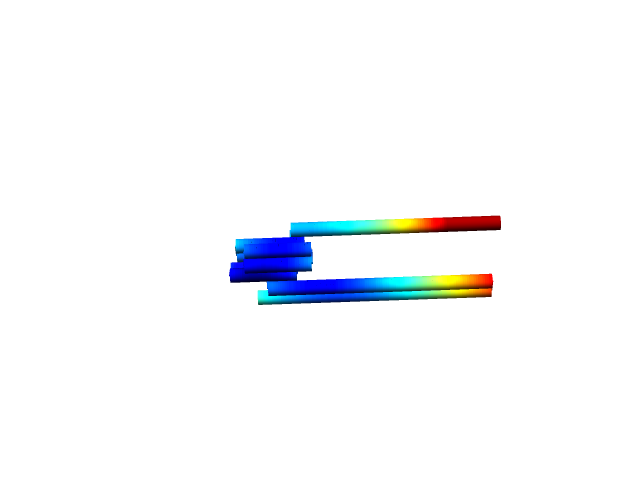
\includegraphics[width=300pt]{long_heat}
\caption{1- vs 2-helix arms}
  \label{fig:long_heat}
\end{figure}

\begin{figure}
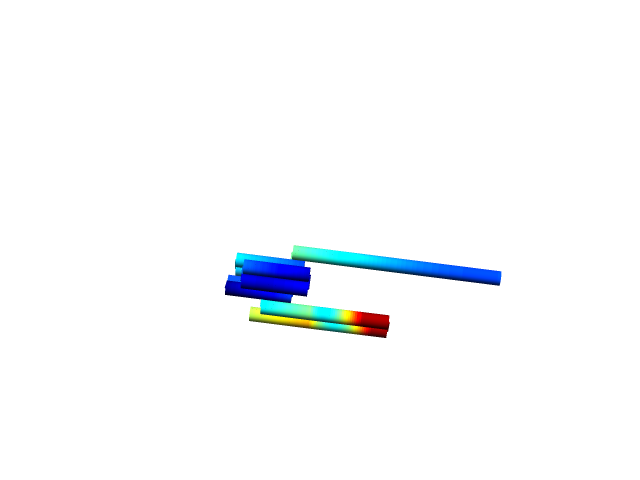
\includegraphics[width=300pt]{short_heat}
\caption{1- vs 2-helix arms}
  \label{fig:short_heat}
\end{figure}

\begin{figure}
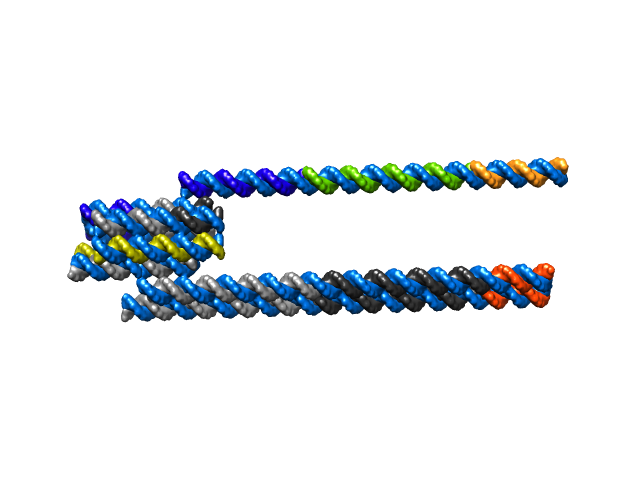
\includegraphics[width=300pt]{long_atomic}
\caption{1- vs 2-helix arms}
  \label{fig:long_atomic}
\end{figure}

\begin{figure}
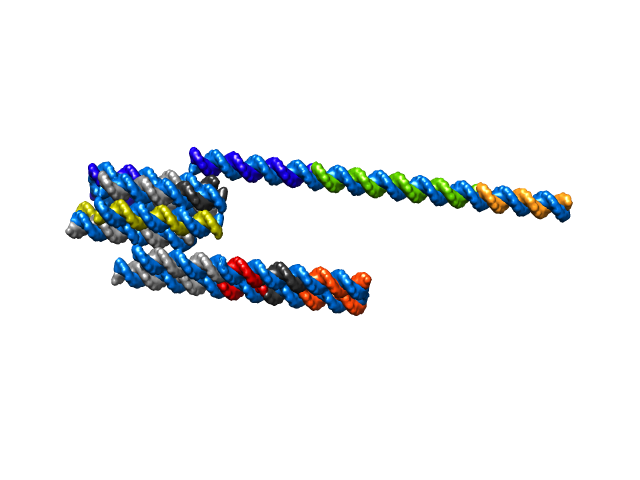
\includegraphics[width=300pt]{short_atomic}
\caption{1- vs 2-helix arms}
  \label{fig:short_atomic}
\end{figure}


\subsection{Effect of doubling width of robot arm}
The heatmap revealed greater flexibility in the 2-helix limb as compared to the single-helix limb. 
\begin{figure}
    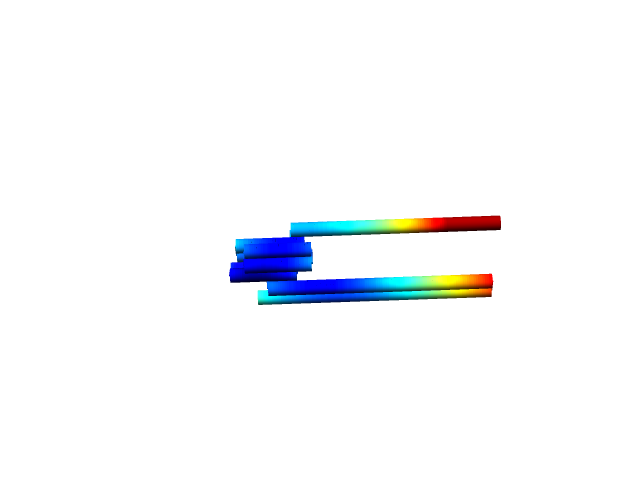
\includegraphics[width=300pt]{single_arm_vs_double_heat}
  \caption{1- vs 2-helix arms}
  \label{fig:single_arm}
\end{figure}

\begin{figure}
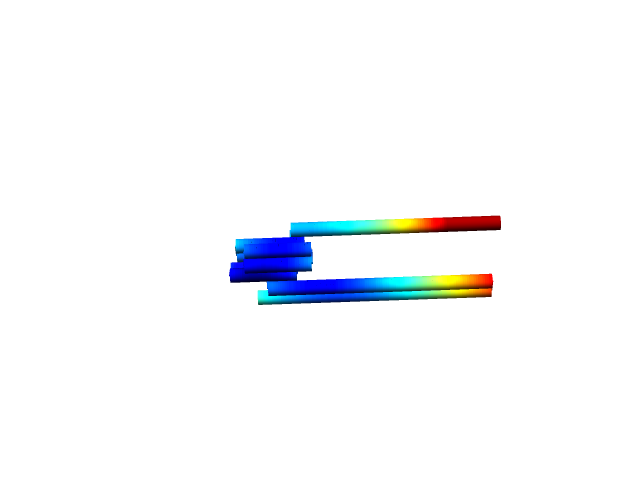
\includegraphics[width=300pt]{single_arm_vs_double_heat}
\caption{1- vs 2-helix arms}
  \label{fig:single_arm2}
\end{figure}

\begin{figure}
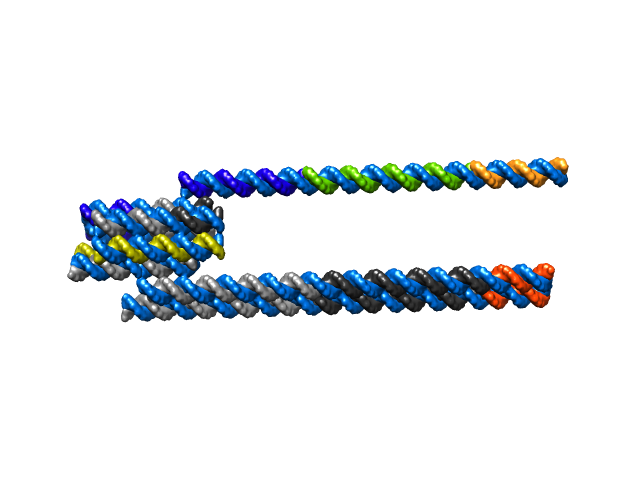
\includegraphics[width=300pt]{single_arm_vs_double_atomic}
\caption{1- vs 2-helix arms in atomic resolution}
  \label{fig:single_arm3}
\end{figure}

\section{Appendix}
\subsection{Design documents}


\subsubsection{Final (long arm)}
\lstinputlisting[breaklines]{final_more_stapled.csv}
\subsubsection{Final (long arm) staples}

\lstinputlisting[breaklines]{final_more_stapled.json}



\subsubsection{Final (short arm)}
\lstinputlisting[breaklines]{final_less_stapled.csv}
\subsubsection{Final (short arm) staples}
\lstinputlisting[breaklines]{final_less_stapled.json}


\begin{thebibliography}{9}

\bibitem{DN}
    DN Kim, F Kilchherr, H Dietz, M Bathe. Quantitative prediction of 3D solution shape and flexibility of nucleic acid nanostructures. Nucleic Acids Research, 40(7):2862-2868 (2012).

\bibitem{Castro}
    CE Castro, F Kilchherr, DN Kim, EL Shiao, T Wauer, P Wortmann, M Bathe, H Dietz. A primer to scaffolded DNA origami. Nature Methods, 8: 221-229 (2011).

\end{thebibliography}

\end{document}

